\chapter{VCO frekvens}
\label{vco-frekvens}

Frekvensen på den VCO som anvendes i volumenkontrollen, se afsnit \ref{volumenkontrol-design-vco}, er afhængig af flere komponenter. Som tidligere nævnt kan den deles op i to blokke; én integrator og én schmidt-trigger. 

\begin{figure}[h]
\centering
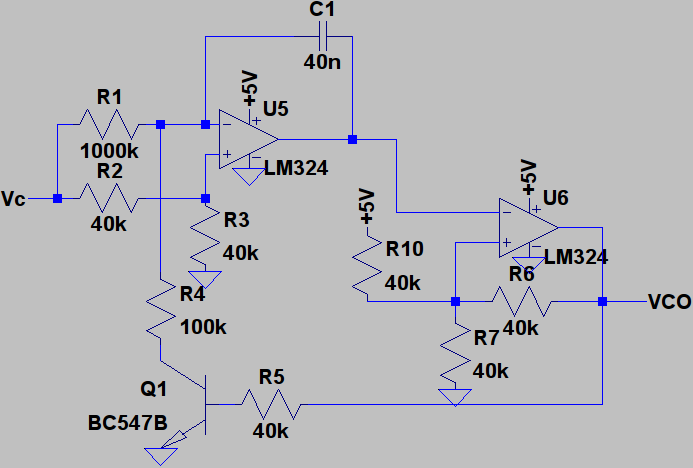
\includegraphics[width=\textwidth]{teknisk/volumenkontrol/vco.png}
\caption{Diagram over VCO'en}
\label{fig:appendiks-vco}
\end{figure}

\subsection*{Schmidt-trigger}

For at opstille et udtryk for frekvensen skal triggerniveauerne for schmidt-triggeren bestemmes, dette gøres vunder den antagelse at et højt udgangs niveau på U6 har samme spænding som forsyningen. Udfra ligning (\ref{equ:appendiks-vco1}) kan $"$Lower triggerlevel$"$ beregnes.

\begin{equation}
\label{equ:appendiks-vco1}
V_L = \frac{R_7||R_6}{R_{10} + R_7||R_6} \cdot V_{CC}
\end{equation}

Hvis de tre modstande $R_6$, $R_7$ og $R_{10}$ gøres ens, kan ligningen yderligere reduceres, se ligning (\ref{equ:appendiks-vco2}).

\begin{equation}
\label{equ:appendiks-vco2}
V_L = \frac{R \cdot R}{R \cdot R + R \cdot R + R \cdot R} \cdot V_{CC} = \frac{1}{3} \cdot V_{CC}
\end{equation}

Da operationsforstærkeren, LM324, ikke er i stand til at levere forsyningsspænding som udgangsspænding, men kun $V_{CC} - 1,5$ V \cite{lm324-datablad}, beregnes $"$Upper triggerlevel$"$ ved at bruges superposition. Udfra ligningerne (\ref{equ:appendiks-vco3a}), (\ref{equ:appendiks-vco3b}) og (\ref{equ:appendiks-vco3d}) kan $"$Upper triggerlevel$"$ beregnes.

\begin{equation}
\label{equ:appendiks-vco3a}
V_{\mathrm{supply}} = \frac{R_6||R_7}{R_{10} + R_6||R_7} \cdot V_{CC}
\end{equation}

\begin{equation}
\label{equ:appendiks-vco3b}
V_{\mathrm{opamp}} = \frac{R_7||R_{10}}{R_6 + R_7||R_{10}} \cdot (V_{CC} - 1,5~\mathrm{V})
\end{equation}

\begin{equation}
\label{equ:appendiks-vco3d}
V_U = V_{\mathrm{supply}} + V_{\mathrm{opamp}} = \frac{R_7 \cdot (R_{10} \cdot V_{CC} + 1,5~\mathrm{V} \cdot R_{10} + R_6 \cdot V_{CC})}{R_6 \cdot R_7 + R_6 \cdot R_{10} + R_7 \cdot R_{10}}
\end{equation}

Når de tre modstande $R_6$, $R_7$ og $R_{10}$ gøres ens, kan ligningen yderligere reduceres, se ligning (\ref{equ:appendiks-vco4}).

\begin{equation}
\label{equ:appendiks-vco4}
V_U = \frac{R \cdot (R \cdot V_{CC} + 1,5~\mathrm{V} \cdot R + R \cdot V_{CC})}{R \cdot R + R \cdot R + R \cdot R} = \frac{2}{3} \cdot V_{CC} - 0,5~\mathrm{V}
\end{equation}

\subsection*{Integrator}
Integratoren op- og aflader kondensatoren $C_1$, dette bliver gjort gennem de to modstande $R_1$ og $R_4$. Med udgangspunkt i den ideelle operationsforstærker, er det klar at spændingen på de to indgange er ens og at operationsforstærkeren vil sikre dette. Det betyder at spændingen på de to indgange kan beregnes med udgangspunkt i $V_+$, se ligning (\ref{equ:appendiks-vco5}).

\begin{equation}
\label{equ:appendiks-vco5}
V_+ = V_- = \frac{R_3}{R_2 + R_3} \cdot V_C
\end{equation}

Ligningen (\ref{equ:appendiks-vco5}) kan reduceres ved at lade modstandene $R_2$ og $R_3$ være ens, se ligning (\ref{equ:appendiks-vco6}).

\begin{equation}
\label{equ:appendiks-vco6}
V_- = \frac{R}{R + R} \cdot V_C = \frac{1}{2} \cdot V_C
\end{equation}

Strømmen gennem $R_1$ kan beregnes udfra $V_C$, $V_-$, den ohmske modstand og Ohms lov, se ligning (\ref{equ:appendiks-vco7}).

\begin{equation}
\label{equ:appendiks-vco7}
V_C - V_- = I_{R_1} \cdot R_1 \Rightarrow I_{R_1} = \frac{V_C - V_-}{R_1} = \frac{V_C - \frac{V_C}{2}}{R_1} = \frac{\frac{V_C}{2}}{R_1} = \frac{V_C}{2 \cdot R_1}
\end{equation}

Når udgangen på $U_6$ er lav vil transistoren $Q_1$ ikke være ledende og der vil ikke løbe strøm gennem $R_4$. Dette vil betyde at al den strøm der løber gennem $R_1$ vil lade $C_1$ op. Altså er $I_{R_1} = I_{\mathrm{op}}$. Når udgangen på $U_6$ er høj vil transistoren $Q_1$ være ledende og der vil løbe en strøm gennem $R_4$. Dette vil betyde at al den strøm der løber gennem $R_1$ vil løbe til stel gennem $R_4$. Da strømmen gennem $R_4$ større end strømmen gennem $R_1$, dette skyldes at der også løber strøm fra kondensatoren til stel, det er denne strøm der aflader kondensatoren. For at beregne strømmen $I_{R_4}$ bruges $V_-$ igen, se ligning (\ref{equ:appendiks-vco8}).

\begin{equation}
\label{equ:appendiks-vco8}
V_- = I_{R_4} \cdot R_4 \Rightarrow I_{R_4} = \frac{V_-}{R_4} = \frac{\frac{V_C}{2}}{R_4} = \frac{V_C}{2 \cdot R_4}
\end{equation}

Da $I_{R_4}$ er summen af opladnings- og afladningsstrømmen kan afladningsstrømmen findes ved ligning (\ref{equ:appendiks-vco9}).

\begin{equation}
\label{equ:appendiks-vco9}
I_{\mathrm{af}} = I_{R_4} - I_{\mathrm{op}} = \frac{V_C}{2 \cdot R_4} - \frac{V_C}{2 \cdot R_1}
\end{equation}

Den spænding kondensatoren skal op- og aflade er forskellen mellem $V_U$ og $V_L$, dette skyldes at det er disse to spændinger udgangen på $U_5$ vil svinge i mellem. Se ligning (\ref{equ:appendiks-vco10})

\begin{equation}
\label{equ:appendiks-vco10}
V_d = \left(\frac{2}{3} \cdot V_{CC} - 0,5~\mathrm{V}\right) - \frac{1}{3} \cdot V_{CC} = \frac{1}{3} \cdot V_{CC} - 0,5~\mathrm{V}
\end{equation}

Tiden det tager at op og aflade kondensatoren beregnes ud fra ligning (\ref{equ:appendiks-vco11}).

\begin{equation}
\label{equ:appendiks-vco11}
V = \frac{I \cdot t}{C} \Rightarrow t = \frac{V \cdot C}{I}
\end{equation}

Udfra ligning (\ref{equ:appendiks-vco11}) kan både op- og afladningstiden beregnes, se ligning (\ref{equ:appendiks-vco12}) og (\ref{equ:appendiks-vco13}).

\begin{equation}
\label{equ:appendiks-vco12}
t_{\mathrm{op}} = \frac{V_d \cdot C}{I_{\mathrm{op}}} = \frac{\left(\frac{1}{3} \cdot V_{CC} - 0,5~\mathrm{V}\right) \cdot C}{\frac{V_C}{2 \cdot R_1}} = \frac{(2 \cdot V_{CC} - 3~\mathrm{V}) \cdot C \cdot R_1}{3 \cdot V_C}
\end{equation}

\begin{equation}
\label{equ:appendiks-vco13}
t_{\mathrm{af}} = \frac{V_d \cdot C}{I_{\mathrm{af}}} = \frac{\left(\frac{1}{3} \cdot V_{CC} - 0,5~\mathrm{V}\right) \cdot C}{\frac{V_C}{2 \cdot R_4} - \frac{V_C}{2 \cdot R_1}} = \frac{(2 \cdot V_{CC} - 3~\mathrm{V}) \cdot C \cdot R_4 \cdot R_1}{3 \cdot V_C \cdot (R_1 - R_4)}
\end{equation}

Periode tiden, $T$, er summen af op- og afladningstiden, se ligning (\ref{equ:appendiks-vco14a}).

\begin{equation}
\label{equ:appendiks-vco14a}
T = t_{\mathrm{op}} + t_{\mathrm{af}} = \frac{(2 \cdot V_{CC} - 3~\mathrm{V}) \cdot C \cdot R_1}{3 \cdot V_C} + \frac{(2 \cdot V_{CC} - 3~\mathrm{V}) \cdot C \cdot R_4 \cdot R_1}{3 \cdot V_C \cdot (R_1 - R_4)}
\end{equation}

Udtrykkket i ligning (\ref{equ:appendiks-vco14a}), kan reduceres til udtrykket vist i ligning (\ref{equ:appendiks-vco14b}).

\begin{equation}
\label{equ:appendiks-vco14b}
T = \frac{(2 \cdot V_{CC} - 3~\mathrm{V}) \cdot C \cdot (R_1)^2}{3 \cdot V_C \cdot (R_1 - R_4)}
\end{equation}

Den frekvens VCO'en vil svinge med beregnes udfra at $f = \frac{1}{T}$, se ligning (\ref{equ:appendiks-vco15}).

\begin{equation}
\label{equ:appendiks-vco15}
f = \frac{1}{T} = \frac{1}{\frac{(2 \cdot V_{CC} - 3~\mathrm{V}) \cdot C \cdot (R_1)^2}{3 \cdot V_C \cdot (R_1 - R_4)}} = \frac{3 \cdot V_C \cdot (R_1 - R_4)}{(2 \cdot V_{CC} - 3~\mathrm{V}) \cdot C \cdot (R_1)^2}
\end{equation}

Den duty cycle som VCO'ens output vil have er reduceret til udtrykket givet i ligning (\ref{equ:appendiks-vco16}).

\begin{equation}
\label{equ:appendiks-vco16}
d = \frac{t_{\mathrm{af}}}{T} = \frac{R_4}{R_1}
\end{equation}